\documentclass{article}
\usepackage{graphicx} % Required for inserting images
\usepackage{amsmath}
\usepackage{amssymb}
\usepackage{float}
\usepackage{textgreek}
\usepackage{fancyhdr}
\usepackage{hyperref}

% vnořené popisky obrázků
\usepackage{subcaption}

% automatická konverze EPS 
\usepackage{graphicx} 
\usepackage{epstopdf}

\pagestyle{fancy}


\newcommand\mat[1]{\begin{bmatrix}#1\end{bmatrix}}
\newcommand\pdiff[2]{\frac{\partial #1}{\partial #2}}
\newcommand\hw[1]{\stepcounter{section}\section*{Úkol \thesection\quad #1}}

\title{ARI-HW\_01}
\author{Matěj Pinkas}
\date{21. February 2024}

\lhead{Pinkas Matěj}
\chead{ARI-HW\_01}
\rhead{21. February 2024}

\begin{document}

\maketitle

\hw{}


\begin{enumerate}
    
    %1.1
    \item Identifikace dat
        \begin{itemize}
            \item[-] Vstupem systému je síla působící na něj ($F$). Vnitřní stavové proměnné jsou rychlost a úhlová rychlost ($v$ a $\omega$). Výsupem systému je měřená rychlost ($v$)
        \end{itemize}
        \begin{align*}
            x &= \mat{v\\ \omega}\\
            u &= F\\
            y &= v
        \end{align*}
    
    %1.2
    \item Implementace modelu
    \begin{figure}[H]
        \centering
        \includegraphics[clip,trim=6.1cm 7.2cm 6.1cm 7.2cm, width=1.00\textwidth]{Figures/ARI_HW1_Circuit_1.pdf}
        \caption{Matematický model 1}
        \label{fig:Model_1}
    \end{figure}


    \newpage
    %1.3
    \item Linearizace modelu pro $v$ = 0 m/s
        \begin{enumerate}
            %1.3.a
            \item Analitická podmínka
                \label{1.3.a}
                \begin{align*}
                    \dot{v} &= -5 \cdot v + \omega + 0.1 \cdot |F|\\
                    \dot{\omega} &= v - \omega
                \end{align*}
                Řešení:
                \begin{align*}
                    \dot{v} &= 0\\
                    \dot{\omega} &= 0\\
                    v &= 0\\ 
                    \\
                    0 &= -5 \cdot 0 + \omega + 0.1 \cdot |F|\\
                    0 &= 0 - \omega\\
                    \\
                    \omega &= 0\\
                    0 &= -5 \cdot 0 + 0 + 0.1 \cdot |F|\\
                    \\
                    |F| &= 0\\
                    \\
                    (v,\omega,F) &= (0,0,0)
                \end{align*}
            %1.3.b
            \item Linearizace v pracovním bodě
                \begin{enumerate}
                    %1.3.b.I
                    \item Se statickou nelinearitou
                        \label{1.3.b.I}
                        \begin{itemize}
                            \item[-] Absolutní hodnota $\left |F \right |$ není diferencovatelná na okolí 0, z toho plyne že linearizovaný model s uváženou statickou nelinearitou není možný zkonstruovat
                        \end{itemize}
                        
                    \newpage
                    %1.3.b.II
                    \item Bez statické nelineartiy
                        \label{1.3.b.II}
                        \begin{itemize}
                            \item[-] Po dosazení bodu ($v$, $\omega$, $F$) = (0,0,0):
                        \end{itemize}

                        \begin{align*}
                            y &= v\\
                            \dot{x_1} &= -5 \cdot v + \omega + 0,1 \cdot |F|\\
                            \dot{x_2} &= v - \omega\\
                            \\
                            A &= \mat{\pdiff{\dot{x_1}}{v} & \pdiff{\dot{x_1}}{\omega}\\
                                      \pdiff{\dot{x_2}}{v} & \pdiff{\dot{x_2}}{\omega}} 
                               = \mat{-5 & 1\\
                                      1 & -1}\\
                            B &= \mat{\pdiff{\dot{x_1}}{F}\\
                                      \pdiff{\dot{x_2}}{F}}
                               = \mat{0,1\\
                                      0}\\
                            C &= \mat{\pdiff{y}{v} & \pdiff{y}{\omega}}
                               = \mat{1 & 0}\\
                            D &= \mat{\pdiff{y}{F}}
                               = \mat{0}\\
                            \\
                            \Delta \dot x(t) &= A \cdot \Delta x(t) + B \cdot \Delta u(t)\\
                            \Delta y(t) &= C \dot \Delta x(t) + D \cdot \Delta u(t)\\
                            \\
                            \mat{\dot{\Delta v}\\ \dot{\Delta \omega}} &= \mat{-5 & 1\\ 1 & -1} \cdot \mat{\Delta v\\ \Delta \omega} + \mat{0,1\\ 0} \cdot \mat{\Delta F}\\
                            \Delta y &= \mat{1 & 0} \cdot \mat{\Delta v\\ \Delta \omega} + \mat{0} \cdot \mat{\Delta F}\\
                        \end{align*}
    
                        
                \end{enumerate}
            
            %1.3.c
            \item Srovnání linearizovaného a původního modelu
                \begin{enumerate}
                    %1.3.c.I
                    \item Se statickou nelinearitou
                        \begin{itemize}
                            \item[-] Model nelze linearizovat na okolí pracovního bodu viz cv. \underline{\ref{1.3.b.I}}, z toho důvodu není možné porovnávat lineární a nelineární model
                        \end{itemize}

                    \newpage
                    
                    %1.3.c.II
                    \item Bez statické nelineartiy\\
                        \begin{figure}[H]
                    	\centering
                    	\begin{subfigure}[b]{0.45\textwidth}
                    		\includegraphics[width=\textwidth]{Figures/Odezva_1_3_linearni.eps}
                    		\caption{Odezva lineárního modelu}
                    		\label{fig:LinearFig_13cII}
                    	\end{subfigure}
                    	~
                    	\begin{subfigure}[b]{0.45\textwidth}
                    		\includegraphics[width=\textwidth]{Figures/Odezva_1_3_nelinearni.eps}
                    		\caption{Odezva nelineárního modelu}
                    		\label{fig:NonlinearFig_13cII}
                    	\end{subfigure}
                     
                    	\caption{Srovnání odezvy matematického modelu s nulovou počáteční podmínkou}
                    	\label{fig:13cIICompare}
                        \end{figure}
                        
                \end{enumerate}
        \end{enumerate}

    %1.4
    \item Linearizace modelu pro $v$ = 10 m/s
        \begin{enumerate}
        %1.4.a
        \item Analitická podmínka
            \begin{itemize}
                \item[-] Postup výpočtu je stejný jako v \underline{\ref{1.3.a}}, ale s $v$ = 10 m/s
            \end{itemize}

            \begin{align*}
                |F| &= 400 \Rightarrow  F = \pm 400\\
                (v,\omega,F) &= (10,10,-400) & (v,\omega,F) &= (10,10,400)
            \end{align*}

        %1.4.b
        \item Linearizace v pracovním bodě
            \begin{enumerate}
                %1.4.b.I
                \item Se statickou nelinearitou
                    \begin{itemize}
                        \item[-] Zde je možné systém linearizovat, protože pracovní bod je velmi vzdálen nedefinovanému bodu derivace v 0
                        \item[-] Postup výpočtu je stejný jako v \underline{\ref{1.3.b.II}}, zde je dosazen bod (10,10,\textpm 400)
                    \end{itemize}
                
                    
                    \begin{align*}
                        \mat{\dot{\Delta v}\\ \dot{\Delta \omega}} &= \mat{-5 & 1\\ 1 & -1} \cdot \mat{\Delta v\\ \Delta \omega} + \mat{0,1\\ 0} \cdot \mat{\Delta F}\\
                        \Delta y &= \mat{1 & 0} \cdot \mat{\Delta v\\ \Delta \omega} + \mat{0} \cdot \mat{\Delta F}\\
                    \end{align*}

                \newpage
                
                %1.4.b.II
                \item Bez statické nelineartiy
                    \begin{itemize}
                        \item[-] Postup výpočtu je stejný jako v \underline{\ref{1.3.b.II}}, zde je dosazen bod (10,10,\textpm 400)
                    \end{itemize}
                
                    \begin{align*}
                        \mat{\dot{\Delta v}\\ \dot{\Delta \omega}} &= \mat{-5 & 1\\ 1 & -1} \cdot \mat{\Delta v\\ \Delta \omega} + \mat{0,1\\ 0} \cdot \mat{\Delta F}\\
                        \Delta y &= \mat{1 & 0} \cdot \mat{\Delta v\\ \Delta \omega} + \mat{0} \cdot \mat{\Delta F}\\
                    \end{align*}
                    
            \end{enumerate}

        %1.4.c
        \item Srovnání linearizovaného a původního modelu
                \begin{itemize}
                    \item[-] Výstupní charakteristika linearizovaného modelu je téměř stejná jako původního modelu a je tedy vhodný pro použití
                \end{itemize}
                
                \begin{figure}[H]
                    \centering
                    \begin{subfigure}[b]{0.45\textwidth}
                        \includegraphics[width=\textwidth]{Figures/Odezva_1_4_linearni.eps}
                        \caption{Odezva lineárního modelu}
                        \label{fig:LinearFig_14cII}
                    \end{subfigure}
                    ~
                    \begin{subfigure}[b]{0.45\textwidth}
                        \includegraphics[width=\textwidth]{Figures/Odezva_1_4_nelinearni.eps}
                        \caption{Odezva nelineárního modelu}
                        \label{fig:NonlinearFig_14cII}
                    \end{subfigure}

                    \caption{Srovnání odezvy matematického modelu pro počáteční bod (10,10,\textpm 400)}
                    \label{fig:4cIICompare}
                \end{figure}
        
        \end{enumerate}

\end{enumerate}


%-----------------------------------------------------------------------------------------------------

\newpage

\hw{}


\begin{enumerate}
    
    %2.1
    \item Identifikace dat
        \begin{itemize}
            \item[-] Vstupem systému je síla působící na něj ($F$). Vnitřní stavové proměnné jsou rychlost a úhlová rychlost ($v$ a $\omega$). Výsupem systému je měřená rychlost ($v$)
        \end{itemize}
        \begin{align*}
            x &= \mat{v\\ \omega}\\
            u &= F\\
            y &= v
        \end{align*}
    
    %2.2
    \item Implementace modelu
        \begin{figure}[H]
        \centering
        \includegraphics[clip,trim=6cm 7cm 6.1cm 7cm, width=1.00\textwidth]{Figures/ARI_HW1_Circuit_2.pdf}
        \caption{Matematický model 2}
        \label{fig:Model_1}
    \end{figure}


    \newpage
    
    %2.3
    \item Linearizace modelu pro $v$ = 0 m/s
        \begin{enumerate}
            %2.3.a
            \item Analitická podmínka
                \label{2.3.a}
                \begin{align*}
                    \dot{v} &= -5 \cdot v \cdot \omega + 0.1 \cdot |F|\\
                    \dot{\omega} &= v - \omega
                \end{align*}
                Řešení:
                \begin{align*}
                    \dot{v} &= 0\\
                    \dot{\omega} &= 0\\
                    v &= 0\\ 
                    \\
                    0 &= -5 \cdot 0 \cdot \omega + 0.1 \cdot |F|\\
                    0 &= 0 - \omega\\
                    \\
                    \omega &= 0\\
                    0 &= -5 \cdot 0 \cdot 0 + 0.1 \cdot |F|\\
                    \\
                    |F| &= 0\\
                    \\
                    (v,\omega,F) &= (0,0,0)
                \end{align*}
            %2.3.b
            \item Linearizace v pracovním bodě
                \begin{enumerate}
                    %2.3.b.I
                    \item Se statickou nelinearitou
                        \label{2.3.b.I}
                        \begin{itemize}
                            \item[-] Absolutní hodnota $\left |F \right |$ není diferencovatelná na okolí 0, z toho plyne že linearizovaný model s uváženou statickou nelinearitou není možný zkonstruovat
                        \end{itemize}
                        
                    \newpage
                    %2.3.b.II
                    \item Bez statické nelineartiy
                        \label{2.3.b.II}
                        \begin{itemize}
                            \item[-] Po dosazení bodu ($v$, $\omega$, $F$) = (0,0,0):
                        \end{itemize}

                        \begin{align*}
                            y &= v\\
                            \dot{x_1} &= -5 \cdot v \cdot \omega + 0,1 \cdot |F|\\
                            \dot{x_2} &= v - \omega\\
                            \\
                            A &= \mat{\pdiff{\dot{x_1}}{v} & \pdiff{\dot{x_1}}{\omega}\\
                                      \pdiff{\dot{x_2}}{v} & \pdiff{\dot{x_2}}{\omega}} 
                               = \mat{-5 \omega & -5 v\\
                                      1 & -1}\\
                            B &= \mat{\pdiff{\dot{x_1}}{F}\\
                                      \pdiff{\dot{x_2}}{F}}
                               = \mat{0,1\\
                                      0}\\
                            C &= \mat{\pdiff{y}{v} & \pdiff{y}{\omega}}
                               = \mat{1 & 0}\\
                            D &= \mat{\pdiff{y}{F}}
                               = \mat{0}\\
                            \\
                            \Delta \dot x(t) &= A \cdot \Delta x(t) + B \cdot \Delta u(t)\\
                            \Delta y(t) &= C \dot \Delta x(t) + D \cdot \Delta u(t)\\
                            \\
                            \mat{\dot{\Delta v}\\ \dot{\Delta \omega}} &= \mat{0 & 0\\ 1 & -1} \cdot \mat{\Delta v\\ \Delta \omega} + \mat{0,1\\ 0} \cdot \mat{\Delta F}\\
                            \Delta y &= \mat{1 & 0} \cdot \mat{\Delta v\\ \Delta \omega} + \mat{0} \cdot \mat{\Delta F}\\
                        \end{align*}
    
                        
                \end{enumerate}
            
            %2.3.c
            \item Srovnání linearizovaného a původního modelu
                \begin{enumerate}
                    %2.3.c.I
                    \item Se statickou nelinearitou
                        \begin{itemize}
                            \item[-] Model nelze linearizovat na okolí pracovního bodu viz cv. \underline{\ref{2.3.b.I}}, z toho důvodu není možné porovnávat lineární a nelineární model
                        \end{itemize}

                    \newpage
                    
                    %2.3.c.II
                    \item Bez statické nelineartiy\\
                        \begin{figure}[H]
                    	\centering
                    	\begin{subfigure}[b]{0.45\textwidth}
                    		\includegraphics[width=\textwidth]{Figures/Odezva_2_3_linearni.eps}
                    		\caption{Odezva lineárního modelu}
                    		\label{fig:LinearFig_23cII}
                    	\end{subfigure}
                    	~
                    	\begin{subfigure}[b]{0.45\textwidth}
                    		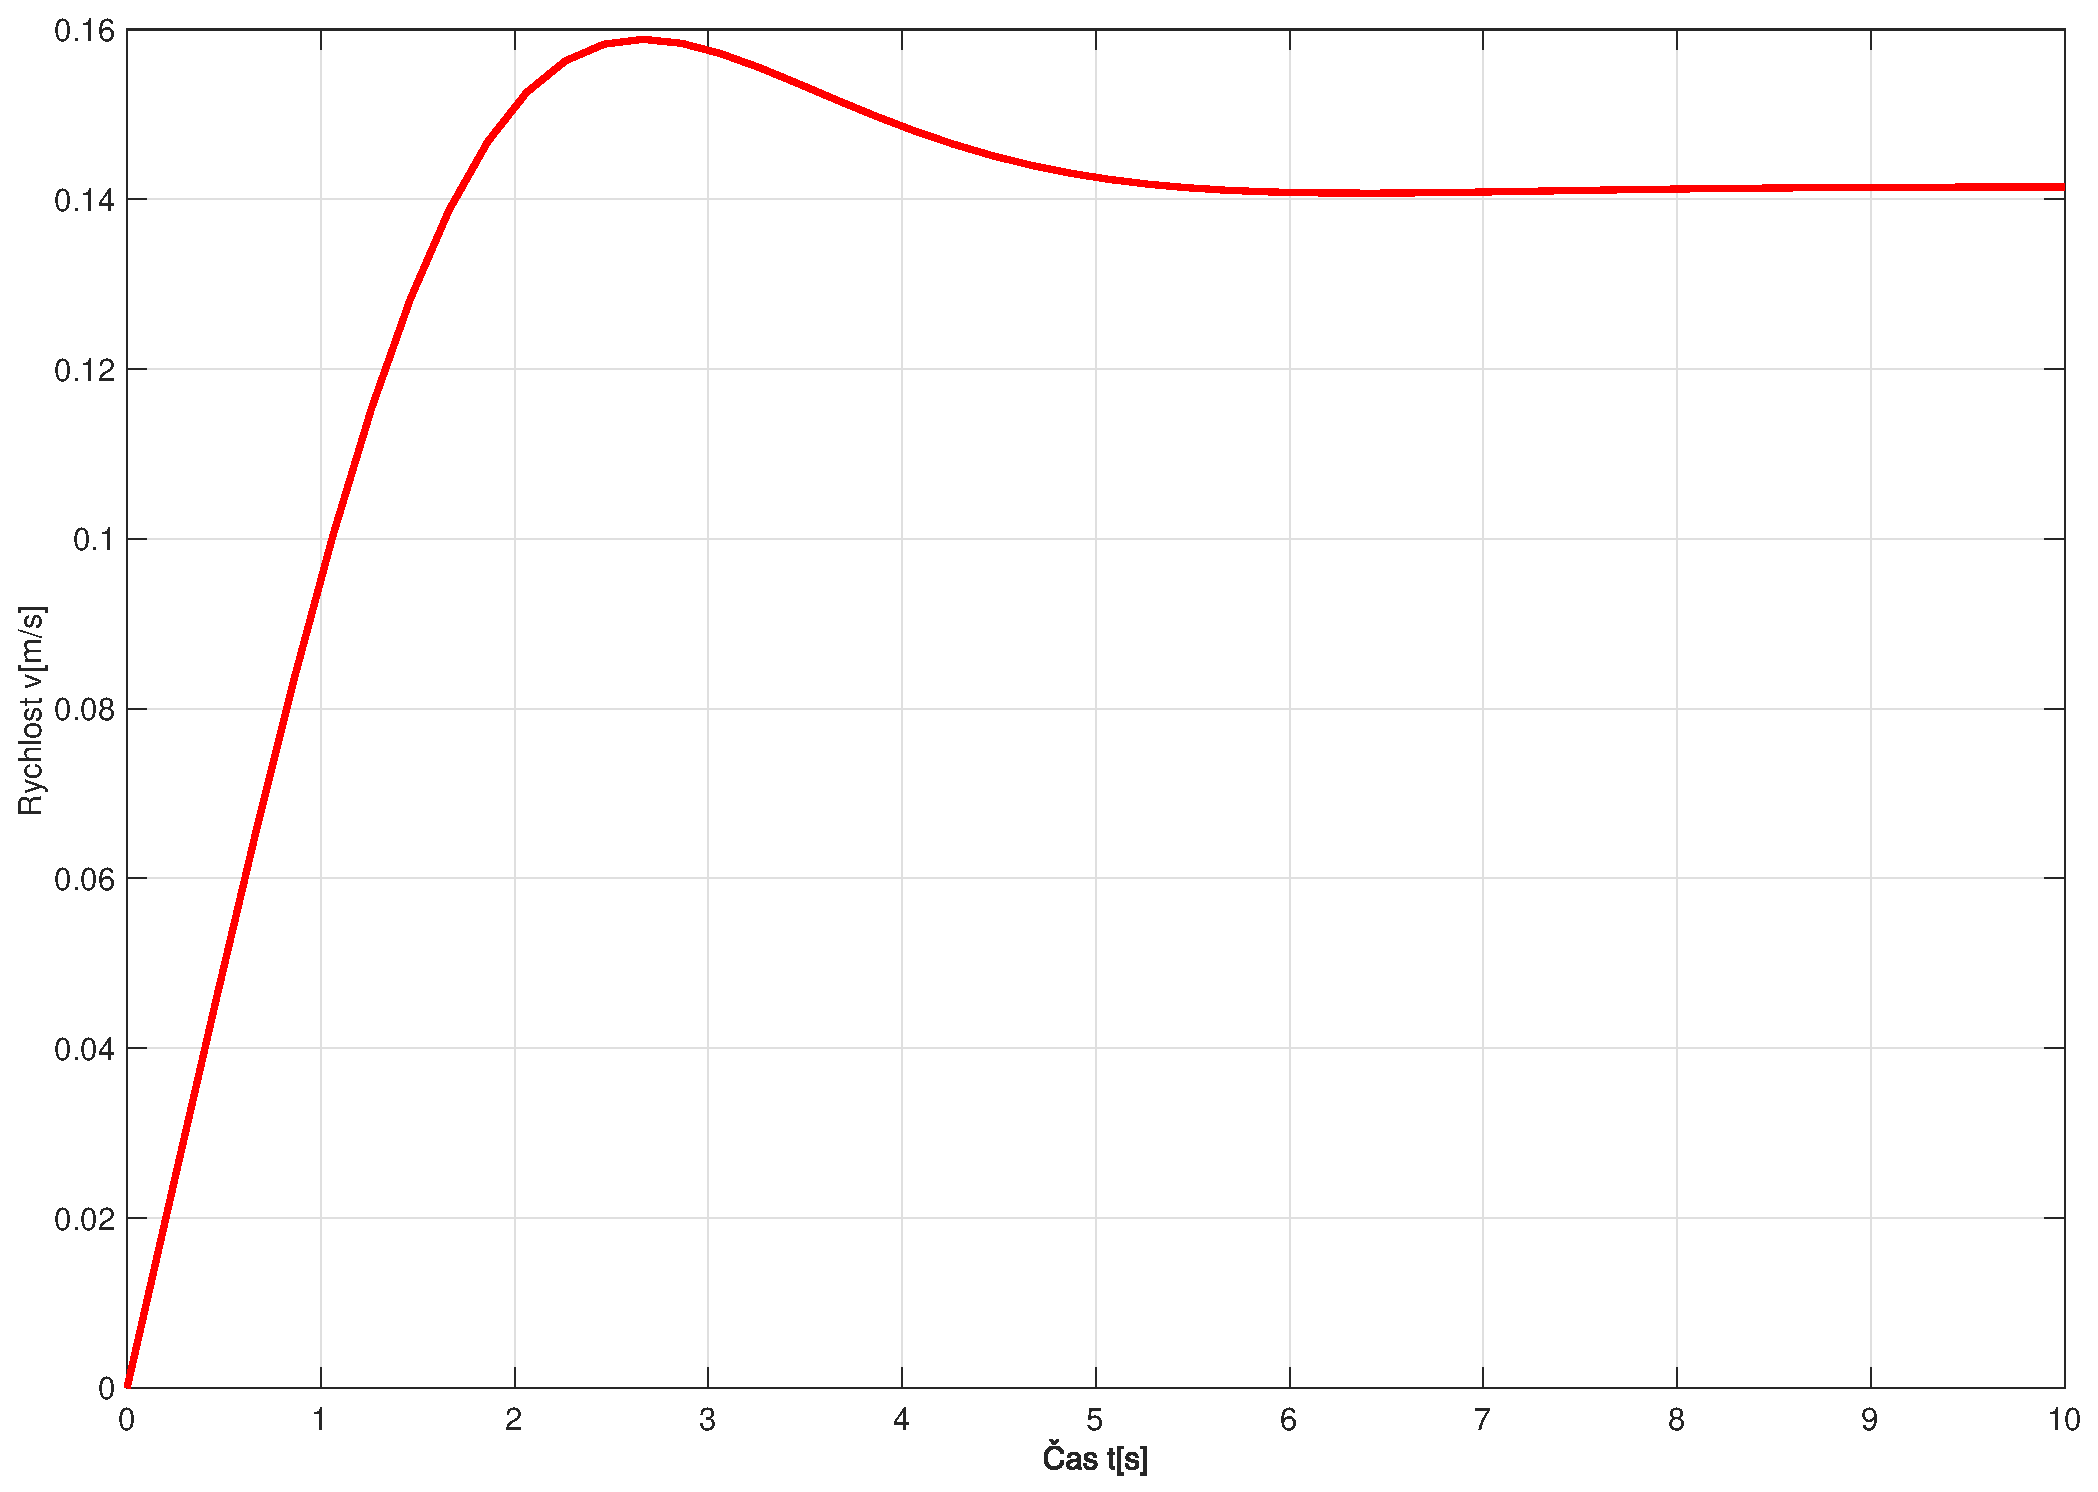
\includegraphics[width=\textwidth]{Figures/Odezva_2_3_nelinearni.eps}
                    		\caption{Odezva nelineárního modelu}
                    		\label{fig:NonlinearFig_23cII}
                    	\end{subfigure}
                     
                    	\caption{Srovnání odezvy matematického modelu s nulovou počáteční podmínkou}
                    	\label{fig:23cIICompare}
                        \end{figure}
                        
                \end{enumerate}
        \end{enumerate}

    %2.4
    \item Linearizace modelu pro $v$ = 10 m/s
    \begin{enumerate}
        %2.4.a
        \item Analitická podmínka
            \begin{itemize}
                \item[-] Postup výpočtu je stejný jako v \underline{\ref{2.3.a}}, ale s $v$ = 10 m/s
            \end{itemize}

            \begin{align*}
                |F| &= 5000 \Rightarrow  F = \pm 5000\\
                (v,\omega,F) &= (10,10,-5000) & (v,\omega,F) &= (10,10,5000)
            \end{align*}

        %2.4.b
        \item Linearizace v pracovním bodě
            \begin{enumerate}
                %2.4.b.I
                \item Se statickou nelinearitou
                    \begin{itemize}
                        \item[-] Zde je možné systém linearizovat, protože pracovní bod je velmi vzdálen nedefinovanému bodu derivace v 0
                        \item[-] Protože jsou zde dva pracovní body budou zde dvě možné linearizace modelu dle každého z pracovních bodů
                        \item[-] Postup výpočtu je stejný jako v \underline{\ref{2.3.b.II}}, zde je dosazen bod (10,10,5000)
                    \end{itemize}
                    
                    \begin{align*}
                        \mat{\dot{\Delta v}\\ \dot{\Delta \omega}} &= \mat{-50 & -50\\ 1 & -1} \cdot \mat{\Delta v\\ \Delta \omega} + \mat{0,1\\ 0} \cdot \mat{\Delta F}\\
                        \Delta y &= \mat{1 & 0} \cdot \mat{\Delta v\\ \Delta \omega} + \mat{0} \cdot \mat{\Delta F}\\
                    \end{align*}

                    \newpage
                    
                    \begin{itemize}
                        \item[-] Postup výpočtu je stejný jako v \underline{\ref{2.3.b.II}}, zde je dosazen bod (10,10,-5000)
                    \end{itemize}
                
                    \begin{align*}
                        \mat{\dot{\Delta v}\\ \dot{\Delta \omega}} &= \mat{-50 & -50\\ 1 & -1} \cdot \mat{\Delta v\\ \Delta \omega} + \mat{-0,1\\ 0} \cdot \mat{\Delta F}\\
                        \Delta y &= \mat{1 & 0} \cdot \mat{\Delta v\\ \Delta \omega} + \mat{0} \cdot \mat{\Delta F}\\
                    \end{align*}
                
                %2.4.b.II
                \item Bez statické nelineartiy
                    \begin{itemize}
                        \item[-] Postup výpočtu je stejný jako v \underline{\ref{2.3.b.II}}, zde je dosazen bod (10,10,\textpm 5000)
                    \end{itemize}
                
                    \begin{align*}
                        \mat{\dot{\Delta v}\\ \dot{\Delta \omega}} &= \mat{-50 & -50\\ 1 & -1} \cdot \mat{\Delta v\\ \Delta \omega} + \mat{0,1\\ 0} \cdot \mat{\Delta F}\\
                        \Delta y &= \mat{1 & 0} \cdot \mat{\Delta v\\ \Delta \omega} + \mat{0} \cdot \mat{\Delta F}\\
                    \end{align*}
                    
            \end{enumerate}

        %2.4.c
        \item Srovnání linearizovaného a původního modelu
                \begin{itemize}
                    \item[-] Výstupní charakteristika linearizovaného modelu je rozdílná oproti původnímu modelu a není tedy příliš vhodná pro použití
                \end{itemize}
                
                \begin{figure}[H]
                    \centering
                    \begin{subfigure}[b]{0.45\textwidth}
                        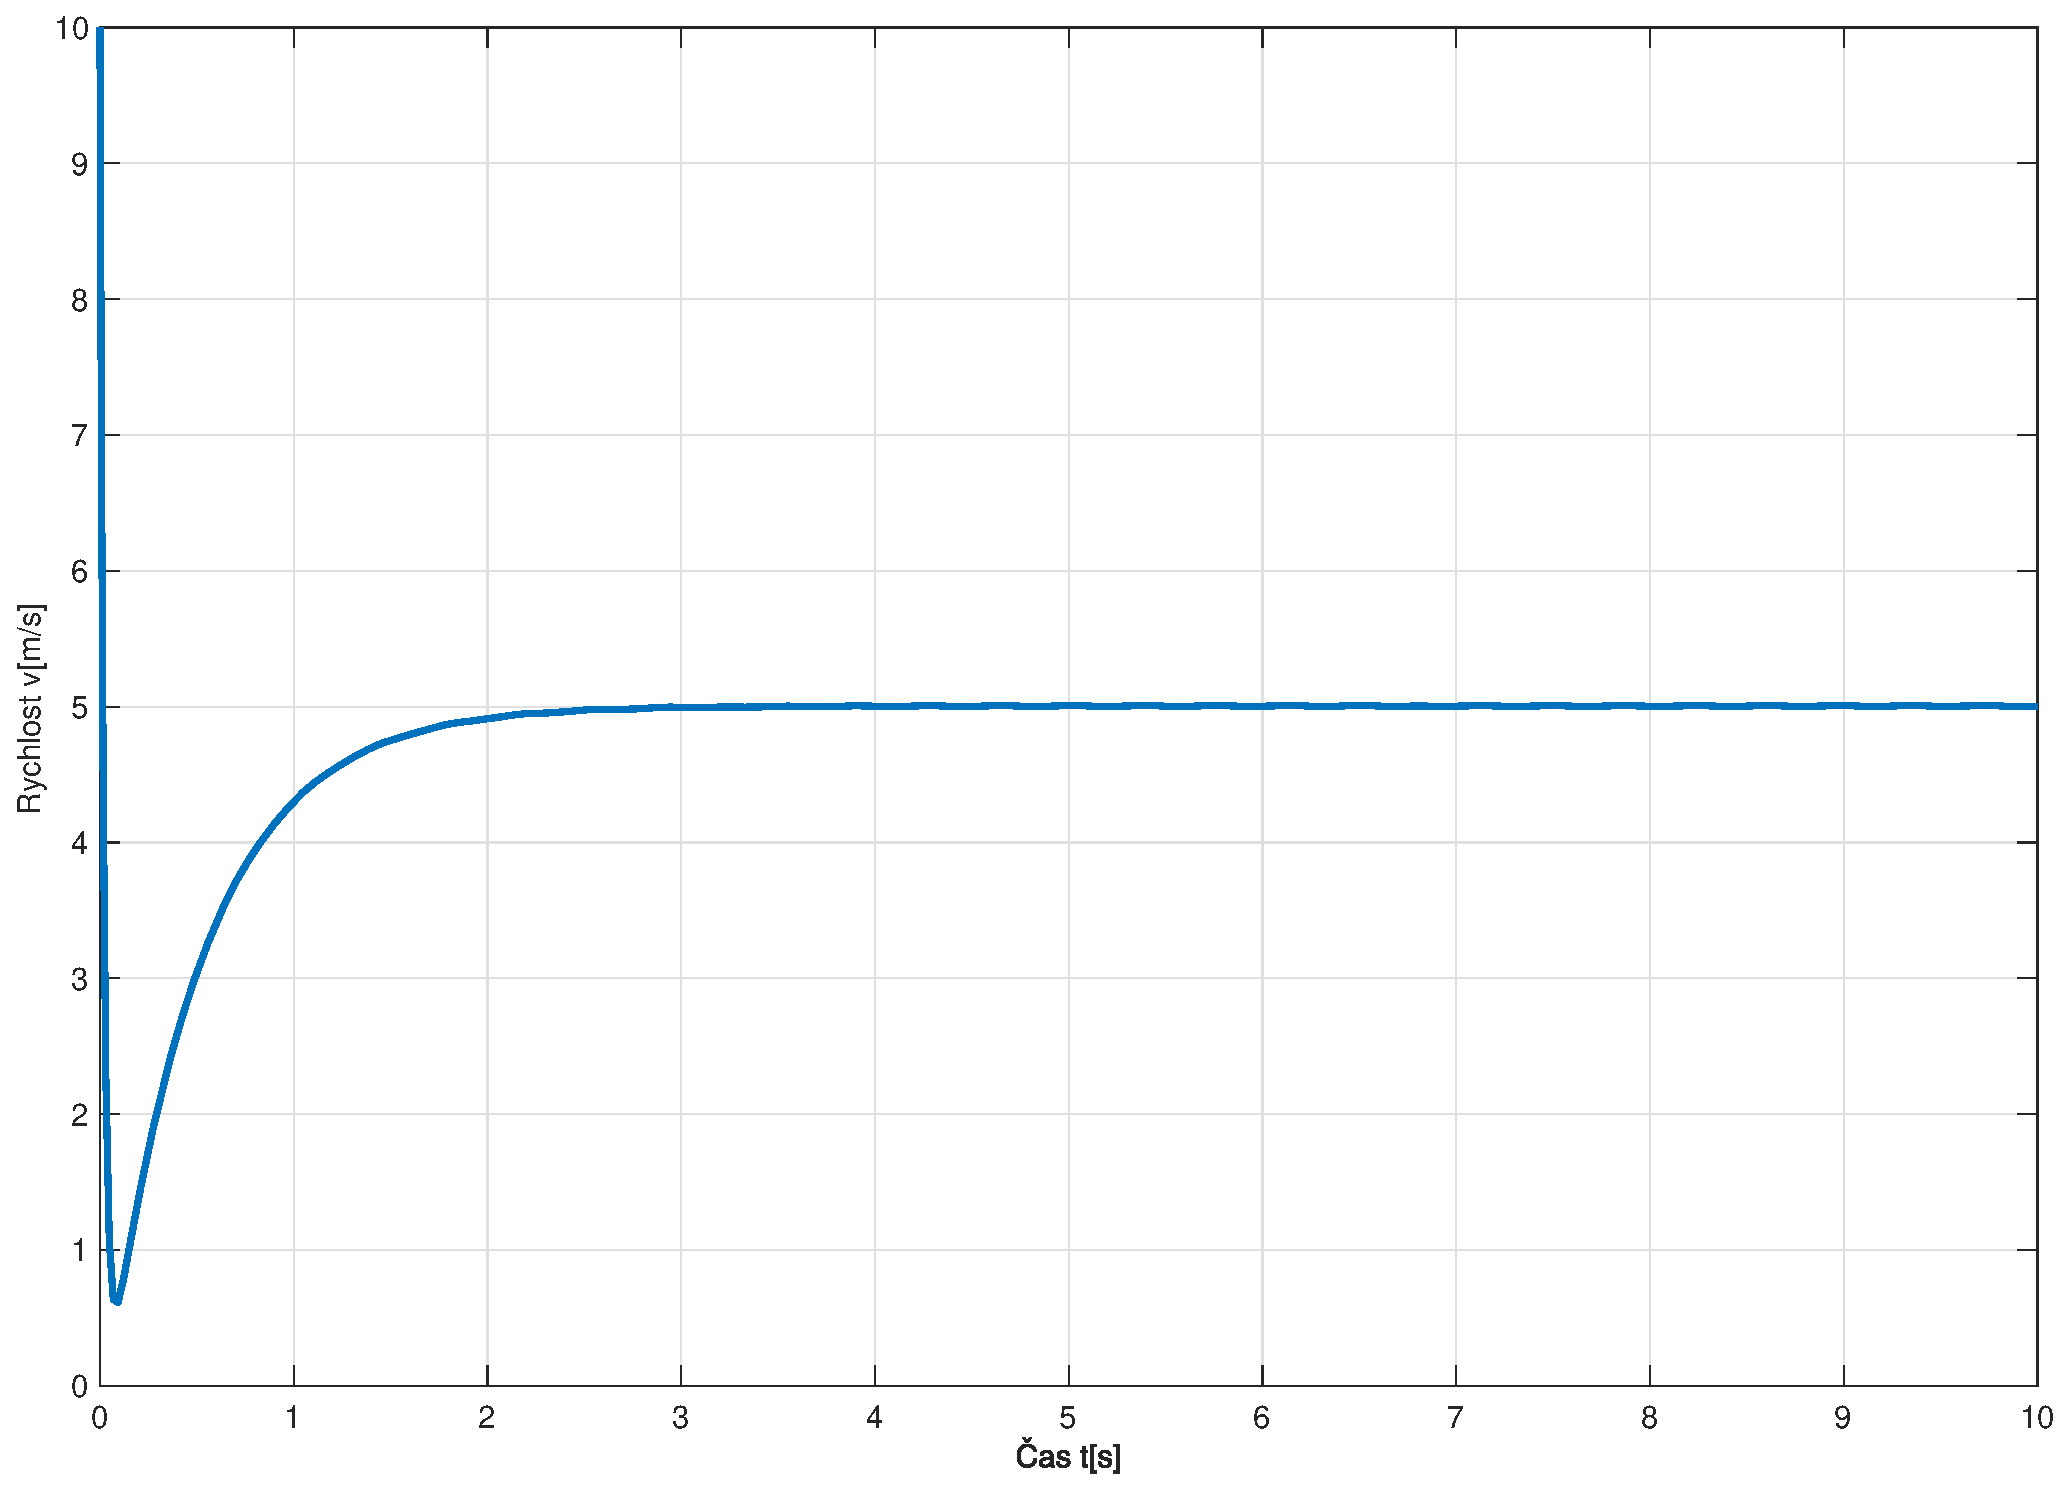
\includegraphics[width=\textwidth]{Figures/Odezva_2_4_linearni.eps}
                        \caption{Odezva lineárního modelu}
                        \label{fig:LinearFig_24cII}
                    \end{subfigure}
                    ~
                    \begin{subfigure}[b]{0.45\textwidth}
                        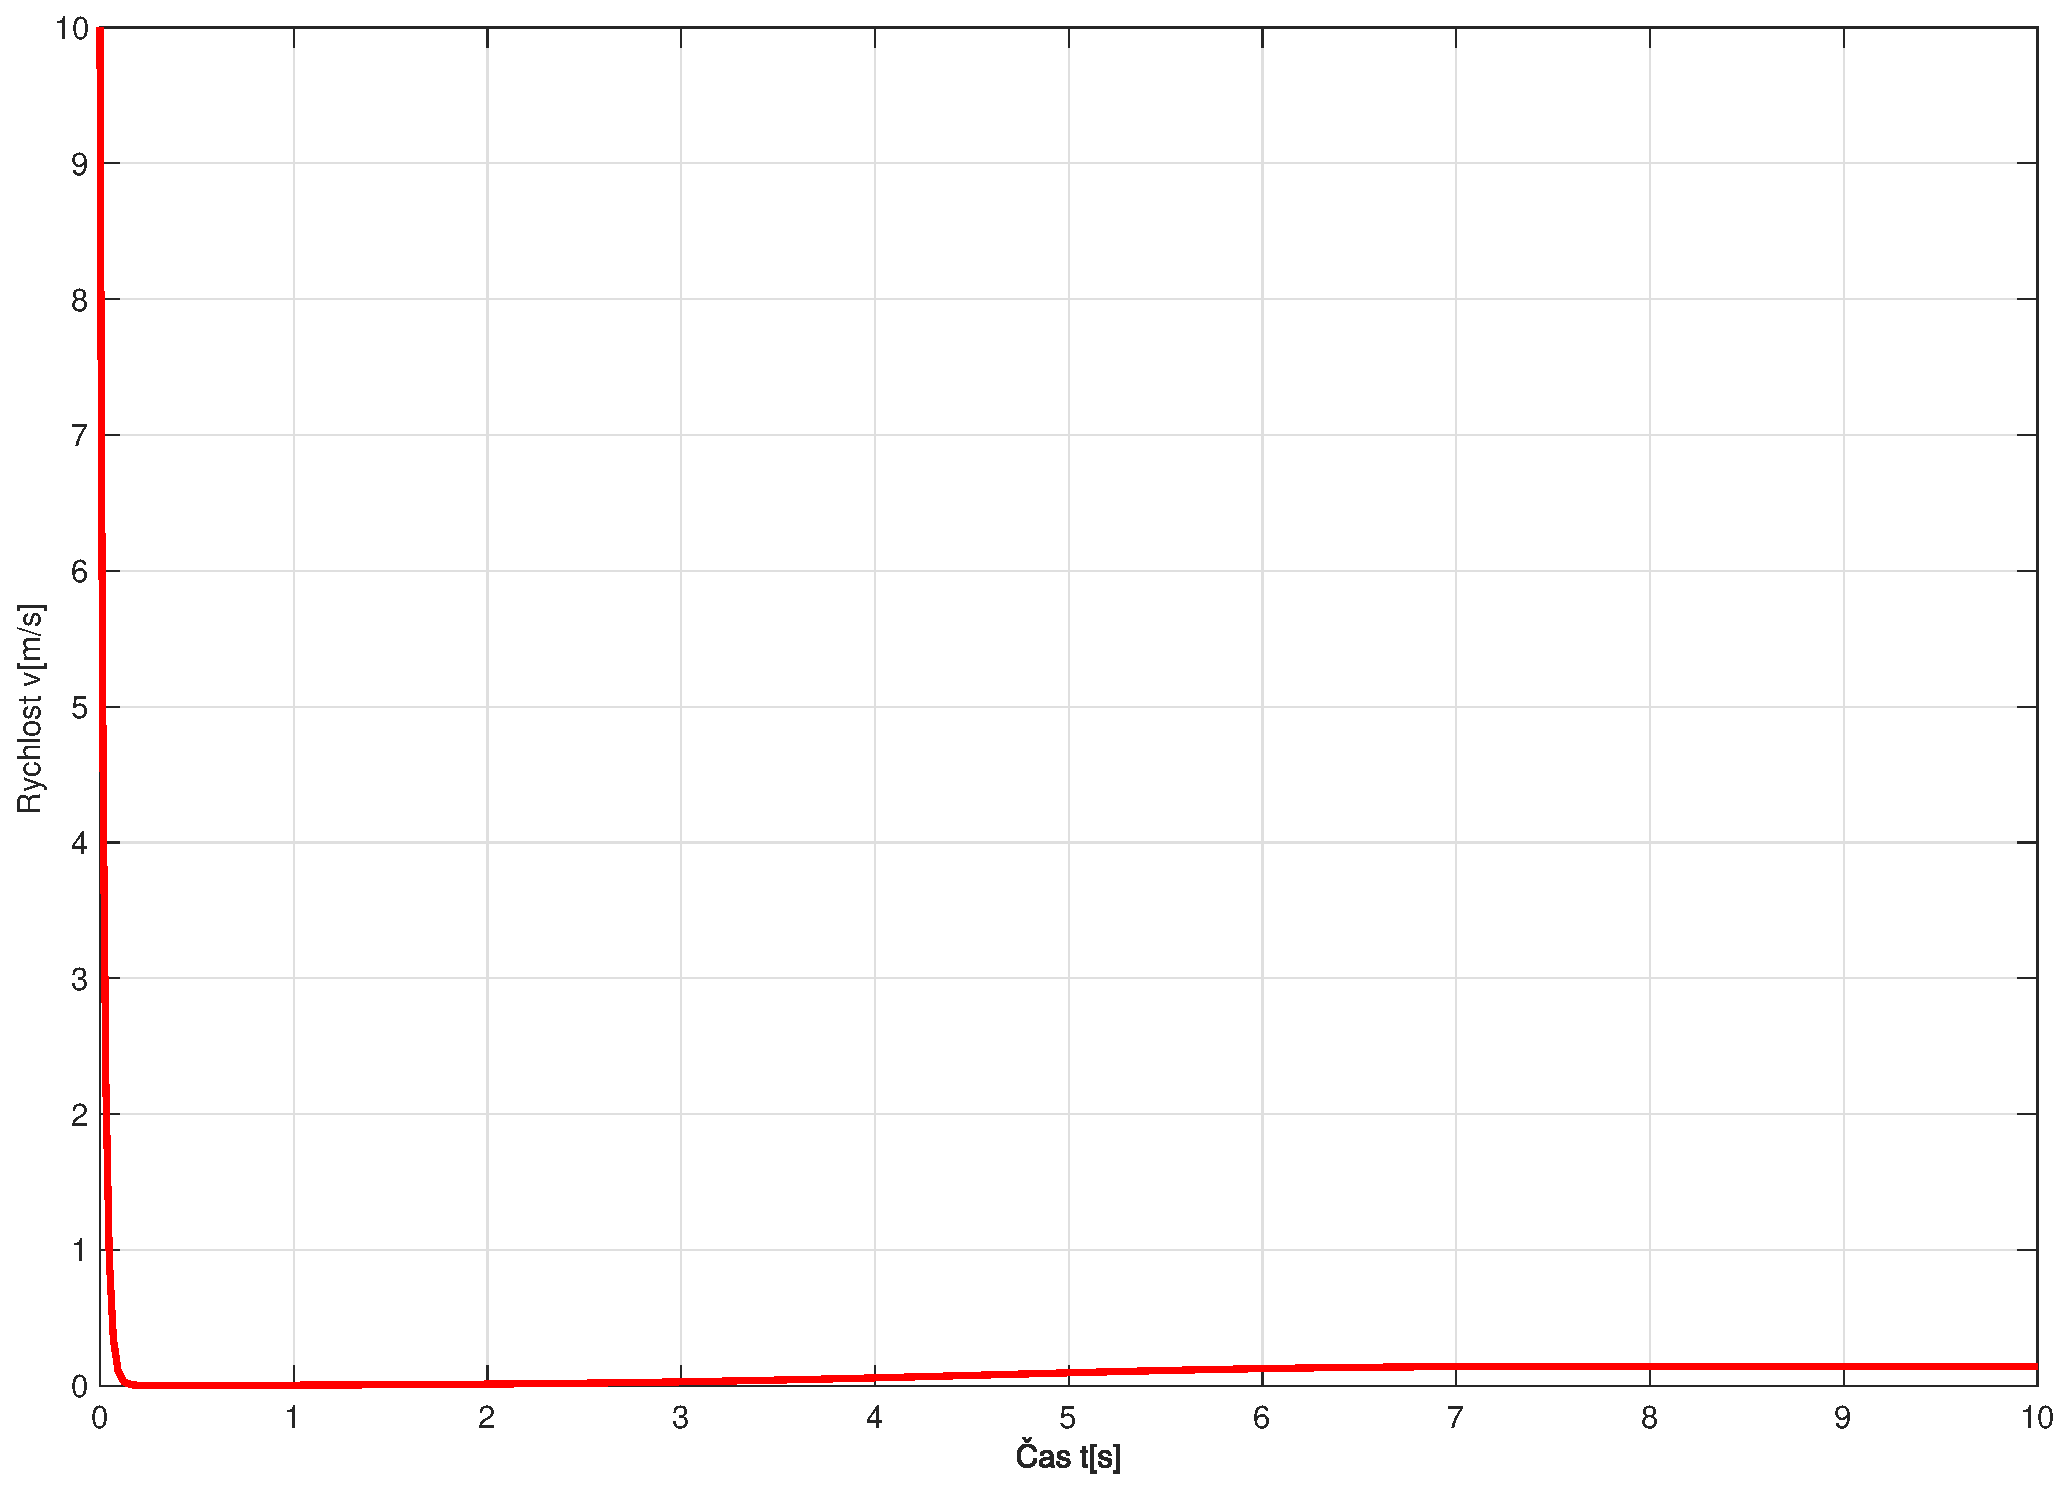
\includegraphics[width=\textwidth]{Figures/Odezva_2_4_nelinearni.eps}
                        \caption{Odezva nelineárního modelu}
                        \label{fig:NonlinearFig_24cII}
                    \end{subfigure}

                    \caption{Srovnání odezvy matematického modelu pro počáteční bod (10,10,\textpm 5000)}
                    \label{fig:24cIICompare}
                \end{figure}
        
        \end{enumerate}

\end{enumerate}


\end{document}
